% ============================================================
% TD : Séries de Fourier
% Pôle Formation UIMM - CVDL - BTS Industriel - S. JAUBERT
% Travaux dirigés (énoncés). Corrigé : MOD13_Series_Fourier_TD_Corrige_v1_0
% ============================================================
\documentclass[a4paper,11pt]{article}
\usepackage[utf8]{inputenc}
\usepackage[T1]{fontenc}
% babel-french absent sur certains postes : chargement conditionnel
\IfFileExists{french.ldf}{\usepackage[french]{babel}}{}
\usepackage{helvet}
\usepackage{courier}
\renewcommand{\familydefault}{\sfdefault}
\usepackage[top=3cm, bottom=2.5cm, left=2cm, right=2cm, headheight=2cm]{geometry}
\usepackage{amsmath,amssymb,amsfonts}
\usepackage{graphicx}
\usepackage[dvipsnames,table]{xcolor}
\usepackage{tikz}
\usetikzlibrary{arrows.meta, positioning}
\usepackage{pgfplots}
\pgfplotsset{compat=1.18}
\usepackage[most]{tcolorbox}
\usepackage{fancyhdr}
\usepackage{enumitem}
\usepackage{array,needspace}
\usepackage{titlesec}
\usepackage{hyperref}

\definecolor{uimmblue}{HTML}{005C85}
\definecolor{uimmred}{HTML}{D31326}
\definecolor{uimmlightblue}{HTML}{E8F1F8}
\definecolor{uimmgray}{HTML}{333333}
\definecolor{uimmlightgray}{HTML}{F5F5F5}
\hypersetup{colorlinks=true, linkcolor=uimmblue, urlcolor=uimmblue}

\titleformat{\section}{\Large\bfseries\color{uimmblue}}{}{0pt}{}[\vspace{2pt}{\color{uimmblue}\titlerule[1.2pt]}]
\setlist[enumerate,1]{label={\color{uimmblue}\textbf{\arabic*.}}}
\setlist[enumerate,2]{label=\alph*)}
\setlist[itemize,1]{label={\color{uimmblue}\textbullet}}

\newtcolorbox{exo}[1]{colback=white, colframe=uimmblue, fonttitle=\bfseries\color{white},
  coltitle=white, title={#1}, boxrule=1pt, arc=2pt,
  left=8pt, right=8pt, top=5pt, bottom=8pt, before skip=10pt, after skip=8pt, breakable}
\newtcolorbox{consigne}{colback=uimmlightgray, colframe=uimmgray, boxrule=0.8pt, arc=3pt,
  left=8pt, right=8pt, top=6pt, bottom=6pt}

\newcommand{\M}[1]{\begin{pmatrix}#1\end{pmatrix}}
\newcommand{\calc}{\,{\color{uimmred}\small\textbf{[calculatrice]}}}
\newcommand{\geo}{\,{\color{uimmred}\small\textbf{[GeoGebra]}}}

\pagestyle{fancy}
\fancyhf{}
\renewcommand{\headrulewidth}{0pt}
\fancyhead[L]{\raisebox{-0.5\height}{
\includegraphics[height=1.5cm]{logo_uimm_placeholder.jpg}}}
\fancyhead[C]{\begin{minipage}{8cm}\centering
  {\small\color{uimmblue}\textbf{Pôle Formation UIMM - CVDL}}\\
  {\footnotesize\color{uimmgray} BTS Industriel -- Mathématiques}\end{minipage}}
\fancyhead[R]{{\small\color{uimmblue}\textbf{MOD13 -- TD}}}
\fancyfoot[C]{{\color{uimmblue}\rule{\textwidth}{1pt}}\\[2pt]
  {\footnotesize\color{uimmgray} Pôle Formation UIMM -- Centre-Val de Loire \hfill S. JAUBERT \hfill \thepage}}

\begin{document}

\begin{tcolorbox}[colback=uimmblue, colframe=uimmblue, sharp corners, boxrule=0pt,
  left=14pt, right=14pt, top=10pt, bottom=10pt]
{\color{white}\LARGE\bfseries Travaux Dirigés -- MOD13}\\[4pt]
{\color{white}\large Séries de Fourier}
\end{tcolorbox}

\vspace{2pt}
\noindent{\small\begin{tabular}{@{}>{\bfseries\color{uimmblue}}l@{\hspace{8pt}}p{13.8cm}@{}}
Période : & Semestre 4 \\
Séquence [S01] : & Séries numériques et signaux : [C01] séries géométriques, [C02] Riemann, [C03] représenter, [C04] lire période, parité, expression \\
Séquence [S02] : & Fourier et spectre : [C01] coefficients, [C02] parité, [C03] sommes partielles, [C04] identifier, [C05] Parseval, [C06] spectre \\
\end{tabular}}

\begin{consigne}
\textbf{Consignes.} Travailler en radians. Rappels : $\omega = \frac{2\pi}{T}$ ; $a_0 = \frac1T\int_0^T f$ ; $a_n = \frac2T\int_0^T f(t)\cos(n\omega t)\,\mathrm dt$ ; $b_n = \frac2T\int_0^T f(t)\sin(n\omega t)\,\mathrm dt$ ; $\cos(n\pi) = (-1)^n$, $\sin(n\pi) = 0$ ; $A_n = \sqrt{a_n^2+b_n^2}$ ; Parseval : $\frac1T\int_0^T f^2 = a_0^2 + \frac12\sum(a_n^2+b_n^2)$. Les questions marquées \geo{} ou \calc{} se traitent avec l'outil indiqué (fiches en annexe du cours).
\end{consigne}

% ============================================================
\needspace{7cm}
\section{Séries numériques \hfill {\normalsize\color{uimmred}[S01] [C01] [C02]}}

\begin{exo}{Exercice 1 -- Séries géométriques}
\label{exo:1}
Pour chaque série, dire si elle converge et, si oui, calculer sa somme.
\[
\text{(a) } \sum_{n\geq 0}\left(\frac13\right)^n
\qquad
\text{(b) } \sum_{n\geq 0} 1{,}02^n
\qquad
\text{(c) } \sum_{n\geq 0}(-0{,}5)^n
\qquad
\text{(d) } \sum_{n\geq 0} 5\times 0{,}6^n
\qquad
\text{(e) } \sum_{n\geq 1} 0{,}1^n
\]
\end{exo}

\begin{exo}{Exercice 2 -- Vibration amortie du bâti d'une presse}
\label{exo:2}
Après chaque coup de presse, le bâti vibre librement. L'amplitude du $k$\textsuperscript{e} cycle d'oscillation est $A_k = 2\times 0{,}75^{k}$ (en mm), pour $k = 0, 1, 2, \dots$ Pendant un cycle complet d'amplitude $A_k$, un point du bâti parcourt une distance $4A_k$ (aller et retour de part et d'autre de sa position d'équilibre).
\begin{enumerate}[label=\alph*)]
  \item Exprimer la distance totale $D$ parcourue par ce point sous forme d'une série. Justifier qu'elle converge et calculer $D$.
  \item \calc{} À partir de quel cycle l'amplitude devient-elle inférieure à $0{,}01$\,mm ?
\end{enumerate}
\end{exo}

\begin{exo}{Exercice 3 -- Séries de Riemann et amplitudes d'harmoniques}
\label{exo:3}
\begin{enumerate}[label=\alph*)]
  \item Parmi les séries suivantes, lesquelles convergent ?
  \quad $\displaystyle\sum_{n\geq1}\frac{1}{n^{1{,}5}}$ ; \quad $\displaystyle\sum_{n\geq1}\frac{1}{n^{0{,}8}}$ ; \quad $\displaystyle\sum_{n\geq1}\frac{1}{n\sqrt n}$ ; \quad $\displaystyle\sum_{n\geq1}\frac{3}{n^2}$ ; \quad $\displaystyle\sum_{n\geq1}\frac{1}{n}$.
  \item \calc{} Avec un tableur, calculer les sommes partielles $S_{10}$, $S_{100}$ et $S_{1000}$ de $\sum\frac1{n^2}$. Comparer à $\frac{\pi^2}{6}$.
  \item Les amplitudes des harmoniques d'un créneau sont proportionnelles à $\frac1n$ ($n$ impair), celles d'un triangle à $\frac{1}{n^2}$. La somme des amplitudes est-elle finie dans chaque cas ? Et la somme des carrés des amplitudes ?
\end{enumerate}
\end{exo}

% ============================================================
\needspace{7cm}
\section{Signaux périodiques \hfill {\normalsize\color{uimmred}[S01] [C03] [C04]}}

\begin{exo}{Exercice 4 -- Lire un signal}
\label{exo:4}
Pour chacun des trois signaux ci-dessous, donner la période, la fréquence, la parité (paire, impaire, ni l'un ni l'autre), la valeur moyenne lue graphiquement et une expression sur une période ou une demi-période.
\begin{center}
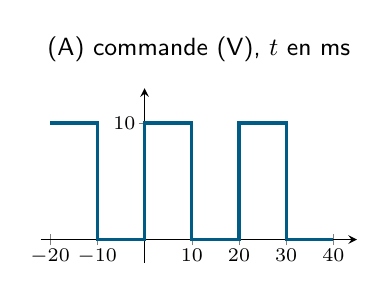
\begin{tikzpicture}[baseline=(current bounding box.north)]
\begin{axis}[width=5.6cm, height=3.8cm, axis lines=middle, xmin=-22, xmax=45, ymin=-2, ymax=13,
  xtick={-20,-10,10,20,30,40}, ytick={10}, title={(A) commande (V), $t$ en ms}, title style={font=\small}, tick label style={font=\scriptsize, fill=white, inner sep=1pt}]
  \addplot[uimmblue, very thick, const plot] coordinates {(-20,10)(-10,0)(0,10)(10,0)(20,10)(30,0)(40,0)};
\end{axis}
\end{tikzpicture}
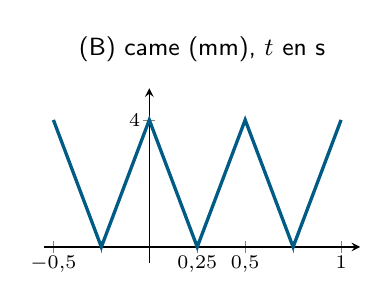
\begin{tikzpicture}[baseline=(current bounding box.north)]
\begin{axis}[width=5.6cm, height=3.8cm, axis lines=middle, xmin=-0.55, xmax=1.1, ymin=-0.5, ymax=5,
  xtick={-0.5,-0.25,0.25,0.5,0.75,1}, xticklabels={$-0{,}5$,,$0{,}25$,$0{,}5$,,$1$}, ytick={4}, title={(B) came (mm), $t$ en s}, title style={font=\small}, tick label style={font=\scriptsize, fill=white, inner sep=1pt}]
  \addplot[uimmblue, very thick] coordinates {(-0.5,4)(-0.25,0)(0,4)(0.25,0)(0.5,4)(0.75,0)(1,4)};
\end{axis}
\end{tikzpicture}
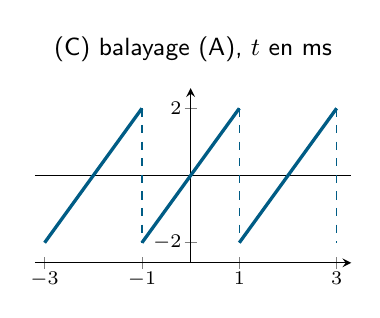
\begin{tikzpicture}[baseline=(current bounding box.north)]
\begin{axis}[width=5.6cm, height=3.8cm, axis x line=bottom, axis y line=middle, xmin=-3.2, xmax=3.3, ymin=-2.6, ymax=2.6,
  xtick={-3,-1,1,3}, ytick={-2,2}, title={(C) balayage (A), $t$ en ms}, title style={font=\small}, tick label style={font=\scriptsize, fill=white, inner sep=1pt}]
  \addplot[black, thin] coordinates {(-3.2,0)(3.3,0)};
  \addplot[uimmblue, very thick] coordinates {(-3,-2)(-1,2)};
  \addplot[uimmblue, very thick] coordinates {(-1,-2)(1,2)};
  \addplot[uimmblue, very thick] coordinates {(1,-2)(3,2)};
  \addplot[uimmblue, dashed] coordinates {(-1,2)(-1,-2)};
  \addplot[uimmblue, dashed] coordinates {(1,2)(1,-2)};
  \addplot[uimmblue, dashed] coordinates {(3,2)(3,-2)};
\end{axis}
\end{tikzpicture}
\end{center}
\end{exo}

\begin{exo}{Exercice 5 -- Courant redressé simple alternance}
\label{exo:5}
Un redresseur à une diode alimente une charge résistive. Le courant, de période $T = 20$\,ms, vaut $i(t) = I\sin(\omega t)$ pour $0\leq t\leq\frac T2$ et $i(t) = 0$ pour $\frac T2\leq t\leq T$, avec $I = 2$\,A.
\begin{enumerate}[label=\alph*)]
  \item Calculer $\omega$. Représenter $i$ sur trois périodes.
  \item Le signal est-il pair ? impair ?
  \item Calculer la valeur moyenne $a_0$ du courant.
\end{enumerate}
\end{exo}

% ============================================================
\needspace{7cm}
\section{Coefficients de Fourier et spectre \hfill {\normalsize\color{uimmred}[S02] [C01] [C02] [C06]}}

\begin{exo}{Exercice 6 -- Signal vibratoire d'un palier du BV12}
\label{exo:6}
Sur le BV12 tournant à $1\,500$\,tr/min, la vitesse vibratoire d'un palier (en mm/s) est modélisée par
\[
v(t) = 1{,}2\sin(50\pi t) + 0{,}9\cos(100\pi t) + 1{,}2\sin(100\pi t) + 0{,}3\sin(150\pi t).
\]
\begin{enumerate}[label=\alph*)]
  \item Déterminer la pulsation $\omega$ du fondamental, la fréquence $f_0$ et la période $T$. Comparer $f_0$ à la fréquence de rotation.
  \item Donner les coefficients $a_0$, $a_n$ et $b_n$ pour $n = 1, 2, 3$ sans calculer d'intégrale.
  \item Calculer les amplitudes $A_1$, $A_2$, $A_3$ et tracer le spectre d'amplitude.
  \item Quelle est la raie dominante ? Quel défaut peut-on suspecter ?
\end{enumerate}
\end{exo}

\begin{exo}{Exercice 7 -- Signal « top-tour » (calcul à la main)}
\label{exo:7}
Un capteur inductif détecte une encoche sur un arbre. Il délivre $E = 24$\,V pendant la première moitié de chaque tour et $0$\,V pendant la seconde : $f(t) = E$ sur $\left]0\,;\,\frac T2\right[$, $f(t) = 0$ sur $\left]\frac T2\,;\,T\right[$.
\begin{enumerate}[label=\alph*)]
  \item Représenter $f$ sur deux périodes et lire sa valeur moyenne.
  \item Calculer $a_0$, puis $a_n$ et $b_n$ pour $n\geq 1$ (distinguer $n$ pair et $n$ impair).
  \item Écrire le début de la série de Fourier (jusqu'à l'harmonique 5) avec des valeurs numériques arrondies au centième.
  \item Montrer que $f - \frac E2$ est un créneau $\pm\frac E2$ et comparer avec le résultat du cours.
\end{enumerate}
\end{exo}

\begin{exo}{Exercice 8 -- Le créneau décalé d'un quart de période}
\label{exo:8}
On considère le créneau $g$ de période $T$ tel que $g(t) = E$ pour $|t| < \frac T4$ et $g(t) = -E$ pour $\frac T4 < |t| < \frac T2$.
\begin{enumerate}[label=\alph*)]
  \item Représenter $g$ sur deux périodes. Montrer graphiquement que $g$ est paire. Quels coefficients sont nuls ?
  \item Montrer que $a_n = \dfrac{4E}{T}\left(\displaystyle\int_0^{T/4}\cos(n\omega t)\,\mathrm dt - \int_{T/4}^{T/2}\cos(n\omega t)\,\mathrm dt\right)$, puis que $a_n = \dfrac{4E}{n\pi}\sin\left(\dfrac{n\pi}{2}\right)$.
  \item Donner $a_1$, $a_2$, $a_3$, $a_4$, $a_5$.
  \item Comparer les amplitudes $A_n$ avec celles du créneau impair du cours. Que change un décalage dans le temps ?
\end{enumerate}
\end{exo}

\begin{exo}{Exercice 9 -- Vidange d'une trémie (intégration par parties)}
\label{exo:9}
Le niveau d'une trémie d'alimentation baisse linéairement de $A$ à $0$ pendant une période $T$, puis la trémie est remplie instantanément : $h(t) = A\left(1 - \dfrac tT\right)$ pour $0\leq t < T$, prolongée par périodicité.
\begin{enumerate}[label=\alph*)]
  \item Représenter $h$ sur deux périodes. Calculer $a_0$.
  \item À l'aide d'une intégration par parties, calculer $b_n$.
  \item On admet que $a_n = 0$. Écrire la série de Fourier de $h$ et la comparer à celle de la dent de scie du cours.
\end{enumerate}
\end{exo}

\begin{exo}{Exercice 10 -- Profil de came (au logiciel)}
\label{exo:10}
On reprend la came (B) de l'exercice 4 : $T = 0{,}5$\,s et $c(t) = 4 - 16t$ sur $[0\,;\,0{,}25]$, $c$ paire.
\begin{enumerate}[label=\alph*)]
  \item Justifier que $b_n = 0$ et calculer $a_0$.
  \item \geo{} Calculer $a_n = \dfrac4T\displaystyle\int_0^{T/2} c(t)\cos(n\omega t)\,\mathrm dt$ en calcul formel. Simplifier selon la parité de $n$.
  \item \calc{} Vérifier la valeur de $a_1$ par un calcul approché d'intégrale.
  \item Comparer avec le triangle du cours : $c$ est-il un triangle $\pm E$ augmenté d'une constante ?
\end{enumerate}
\end{exo}

% ============================================================
\needspace{7cm}
\section{Convergence et identification \hfill {\normalsize\color{uimmred}[S02] [C03] [C04]}}

\begin{exo}{Exercice 11 -- Reconstituer le signal top-tour}
\label{exo:11}
On reprend le signal de l'exercice 7 avec $T = 1$ et $E = 24$.
\begin{enumerate}[label=\alph*)]
  \item \geo{} Définir le signal : \texttt{f(x) = Si(x - floor(x) < 0.5, 24, 0)}.
  \item \geo{} Définir un curseur \texttt{N} et la somme partielle \texttt{S(x) = 12 + Somme(48 / (pi (2k - 1)) sin((2k - 1)*2 pi x), k, 1, N)}. Observer $S$ pour $N = 1$, $3$, $10$, $30$.
  \item Que vaut $S(0)$ pour tout $N$ ? Justifier par le théorème de Dirichlet.
  \item Calculer $S\left(\frac14\right)$ pour $N = 1$ et $N = 3$. Vers quelle valeur doit tendre $S\left(\frac14\right)$ ?
\end{enumerate}
\end{exo}

\begin{exo}{Exercice 12 -- Associer signaux et développements}
\label{exo:12}
On considère trois signaux de période $T$ et de pulsation $\omega$ : (1) le créneau top-tour $0/E$ de l'exercice 7 ; (2) la dent de scie montante de $0$ à $A$ du cours ; (3) le triangle pair $\pm E$ du cours. Associer à chacun son développement, en justifiant sans calcul d'intégrale. Un développement est en trop.
\[
\text{(a) } \frac{8E}{\pi^2}\sum_{k\geq 0}\frac{\cos((2k+1)\omega t)}{(2k+1)^2}
\qquad
\text{(b) } \frac E2 + \frac{2E}{\pi}\sum_{k\geq 0}\frac{\sin((2k+1)\omega t)}{2k+1}
\]
\[
\text{(c) } \frac A2 - \frac A\pi\sum_{n\geq 1}\frac{\sin(n\omega t)}{n}
\qquad
\text{(d) } \frac{4E}{\pi}\sum_{k\geq 0}\frac{\cos((2k+1)\omega t)}{2k+1}
\]
\end{exo}

% ============================================================
\needspace{7cm}
\section{Parseval et valeur efficace \hfill {\normalsize\color{uimmred}[S02] [C05] [C06]}}

\begin{exo}{Exercice 13 -- Valeur efficace du triangle}
\label{exo:13}
On considère le triangle pair $\pm E$ du cours : $f(t) = E\left(1 - \frac{4t}{T}\right)$ sur $\left[0\,;\,\frac T2\right]$, et ses coefficients $a_n = \frac{8E}{n^2\pi^2}$ pour $n$ impair, $0$ sinon.
\begin{enumerate}[label=\alph*)]
  \item Calculer la valeur exacte de $\frac1T\int_0^T f^2(t)\,\mathrm dt$ (utiliser la parité et le changement de variable $u = 1-\frac{4t}{T}$, ou le logiciel). En déduire la valeur efficace.
  \item Calculer la part de cette valeur due au seul fondamental. Commenter.
  \item En déduire la somme $\displaystyle\sum_{k\geq 0}\frac{1}{(2k+1)^4}$.
\end{enumerate}
\end{exo}

\begin{exo}{Exercice 14 -- Niveau global vibratoire}
\label{exo:14}
On reprend le signal $v(t)$ de l'exercice 6 (amplitudes en mm/s).
\begin{enumerate}[label=\alph*)]
  \item Calculer la valeur efficace de chaque raie, puis le niveau global $V_{\text{eff}}$ par la formule de Parseval.
  \item Le service maintenance a fixé un seuil d'alerte à $1{,}8$\,mm/s pour ce palier. Faut-il intervenir ?
  \item Après un réalignement, l'amplitude de la raie 2× est divisée par $4$, les autres raies sont inchangées. Calculer le nouveau niveau global. Quel pourcentage de baisse obtient-on ?
\end{enumerate}
\end{exo}

% ============================================================
\needspace{7cm}
\section{Problème de synthèse \hfill {\normalsize\color{uimmred}[S01] [C03] -- [S02] [C01] [C05] [C06]}}

\begin{exo}{Problème -- Signature d'un défaut de roulement (modèle simplifié)}
\label{exo:pb}
Un écaillage sur la bague extérieure d'un roulement provoque un choc à chaque passage d'une bille, soit $f_c = 100$ chocs par seconde. On modélise très simplement l'accélération mesurée par un train d'impulsions rectangulaires de période $T = \frac{1}{f_c}$ : $s(t) = E$ pour $|t| < \frac\tau2$ et $s(t) = 0$ pour $\frac\tau2 < |t| < \frac T2$, avec une durée de choc $\tau = \frac{T}{10}$.
\begin{enumerate}
  \item \textbf{Le signal.}
  \begin{enumerate}
    \item Calculer $T$ et $\tau$ en ms. Représenter $s$ sur deux périodes.
    \item Étudier la parité de $s$. Quels coefficients sont nuls ?
  \end{enumerate}
  \item \textbf{Les coefficients.}
  \begin{enumerate}
    \item Calculer $a_0$ et l'interpréter.
    \item Montrer que $a_n = \dfrac{2E}{n\pi}\sin\left(\dfrac{n\pi}{10}\right)$.
    \item \calc{} Calculer $a_1, \dots, a_{10}$ en fonction de $E$ (arrondis au millième) et tracer le spectre. À quelles fréquences sont les raies ?
  \end{enumerate}
  \item \textbf{Exploitation.}
  \begin{enumerate}
    \item Comparer ce spectre avec celui d'un balourd. Pourquoi parle-t-on d'un « peigne de raies » ?
    \item Calculer la valeur exacte de $\frac1T\int_0^T s^2(t)\,\mathrm dt$. Quelle part de cette puissance est portée par $a_0$ et les $9$ premiers harmoniques ?
    \item Que devient le spectre si les chocs deviennent plus brefs (par exemple $\tau = \frac{T}{20}$) ? Pourquoi l'analyste surveille-t-il les hautes fréquences pour détecter tôt un défaut de roulement ?
  \end{enumerate}
\end{enumerate}
\end{exo}

\end{document}
